\setcounter{page}{1}

\section{Objetivos}
    \begin{itemize}
        \item Explicar la topología física del entorno del laboratorio de redes
        \item Distinguir los componentes necesarios para construir cables de tipo recto y cruzado.
        \item Construir cables de tipo recto y cruzado empleando los estándares adecuados.
        \item Identificar en qué situaciones se empleará cada tipo de cable.
        \item Configurar la IP y máscara de red en computadoras personales; una de ellas trabajando bajo el sistema  operativo Windows y la otra, bajo Linux.
        \item Verificar la conectividad, mediante un enlace directo, entre dos computadoras personales pertenecientes a la misma red.
    \end{itemize}

\section{Introducción}

    %En la actualidad, las redes de computadoras son una herramienta fundamental para la comunicación y el intercambio de información. Para que una red de computadoras funcione correctamente, es necesario que los dispositivos estén conectados de manera adecuada. En este sentido, el cableado estructurado es un elemento fundamental para la correcta transmisión de datos en una red de computadoras.

    %El cableado estructurado es un sistema de cableado que permite la interconexión de dispositivos de red, como computadoras, impresoras, servidores, entre otros. Este sistema de cableado se compone de cables de red, conectores, patch panels, switches, entre otros elementos. Los cables de red son los encargados de transmitir la información entre los dispositivos de la red. Los conectores son los elementos que permiten conectar los cables de red a los dispositivos de la red. Los patch panels son los elementos que permiten interconectar los cables de red en un armario de comunicaciones. Los switches son los elementos que permiten interconectar los dispositivos de la red.

    %En este laboratorio, se realizará la construcción de cables de red de tipo recto y cruzado, siguiendo los estándares T568A y T568B. Los cables de red de tipo recto se utilizan para conectar dispositivos de red del mismo tipo, como una computadora a un switch. Los cables de red de tipo cruzado se utilizan para conectar dispositivos de red de distinto tipo, como dos computadoras directamente.

    %Además, se configurarán las direcciones IP y máscaras de red en dos computadoras personales, una trabajando bajo el sistema operativo Windows y la otra, bajo Linux. Posteriormente, se verificará la conectividad entre las dos computadoras personales, mediante un enlace directo.

    %En resumen, en este laboratorio se realizará la construcción de cables de red de tipo recto y cruzado, la configuración de direcciones IP y máscaras de red en dos computadoras personales, y la verificación de la conectividad entre las dos computadoras personales, mediante un enlace directo.

\section{Marco Teórico}
    \subsection{Cable UTP}

    El cable UTP (Unshielded Twisted Pair) es un tipo de cable de red que se utiliza para la transmisión de datos en redes de computadoras. Este tipo de cable se compone de pares de hilos de cobre trenzados, los cuales están recubiertos por un aislante de plástico. Los pares de hilos están trenzados para reducir las interferencias electromagnéticas entre los hilos dentro del mismo cable y con cables cercanos. El cable UTP es uno de los cables más utilizados en redes de computadoras, debido a su bajo costo y facilidad de instalación.

    El cable UTP, par trenzado sin blindaje pos sus siglas en inglés (UTP), es un cable balanceado sin blindaje con hilos de colores de par trenzado. Este tipo de cable está disponible en versiones de dos y cuatro pares, fue el tipo de cable dominante en el cableado de piso y cableado de terminales en la década de 1990 y forma parte del estándar de cableado 11801 y de las especificaciones EIA / TIA (\cite{Castro_2023}).

    \subsection{Estándares T568A y T568B}
    Los cables de red se componen de cuatro pares de cables, cada uno de los cuales consta de un cable de color sólido y una franja del mismo color. Para la red Ethernet 10/100BASE-T, solo se utilizan dos pares de cables (naranja y verde). Los otros dos pares de cables (de color marrón y azul) se utilizan para otra aplicación de red Ethernet o para conexiones telefónicas.

    \begin{figure}[H]
        \centering
        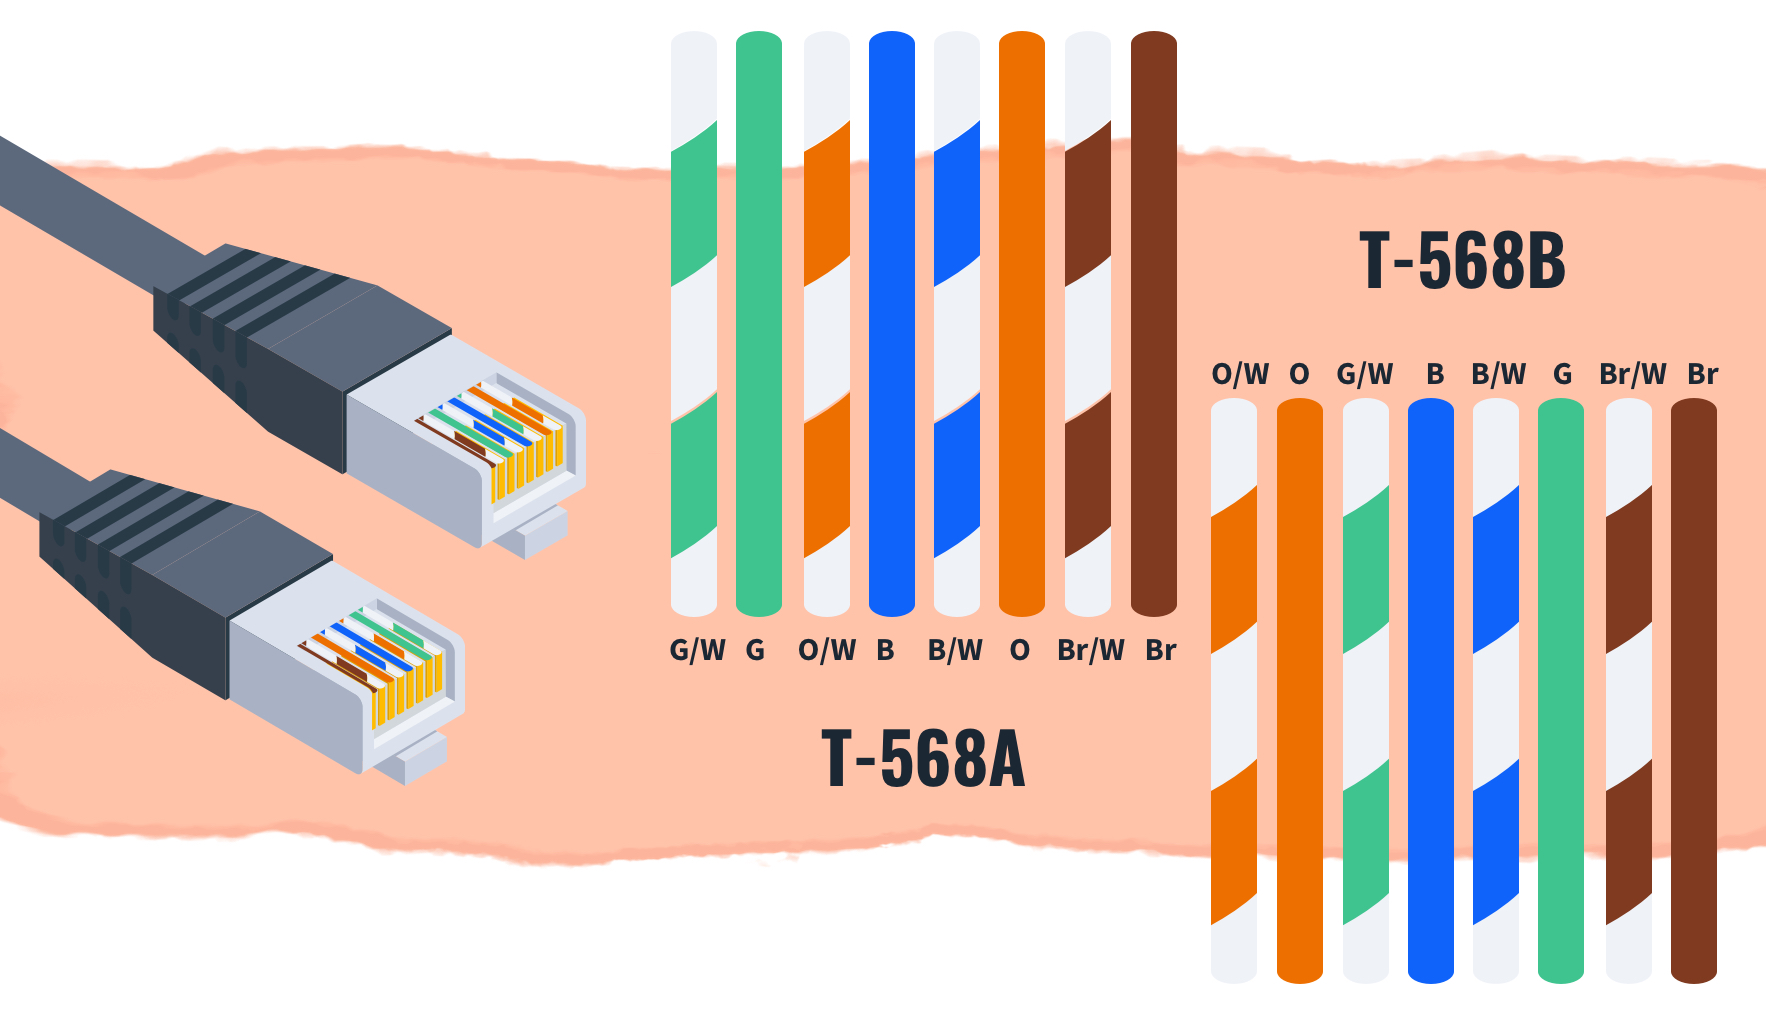
\includegraphics[width=0.6\textwidth]{img/estandar.jpg}
        \caption{Estándar T568A y T568B.}
        \label{fig:estandar}
    \end{figure}

    Como se muestra en la imagen \ref{fig:estandar_t568a_vs_t568b}, existen dos estándares para la disposición de los cables en un conector RJ45: T568A y T568B. Ambos estándares son ampliamente utilizados en la actualidad y son compatibles entre sí.
    Sin embargo la principal diferencia entre estos dos estándares es la posición de los pares de cables naranja y verde.

    \begin{figure}[H]
        \centering
        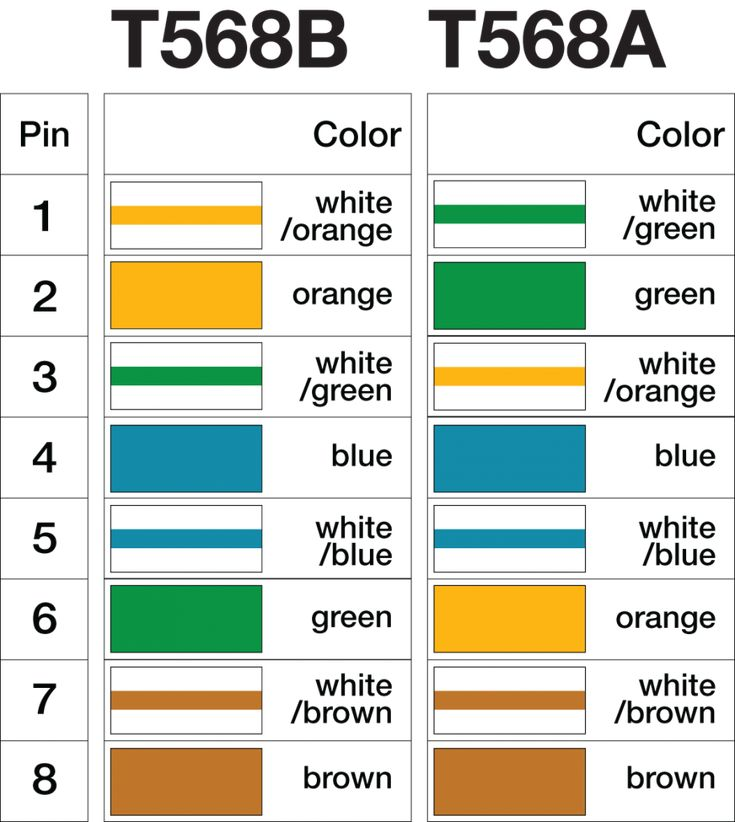
\includegraphics[width=0.6\textwidth]{img/T568AvsT568B.jpg}
        \caption{Estándar T568A vs T568B.}
        \label{fig:estandar_t568a_vs_t568b}
    \end{figure}

    \begin{figure}[H]
        \centering
        \begin{minipage}[b]{0.45\linewidth}
            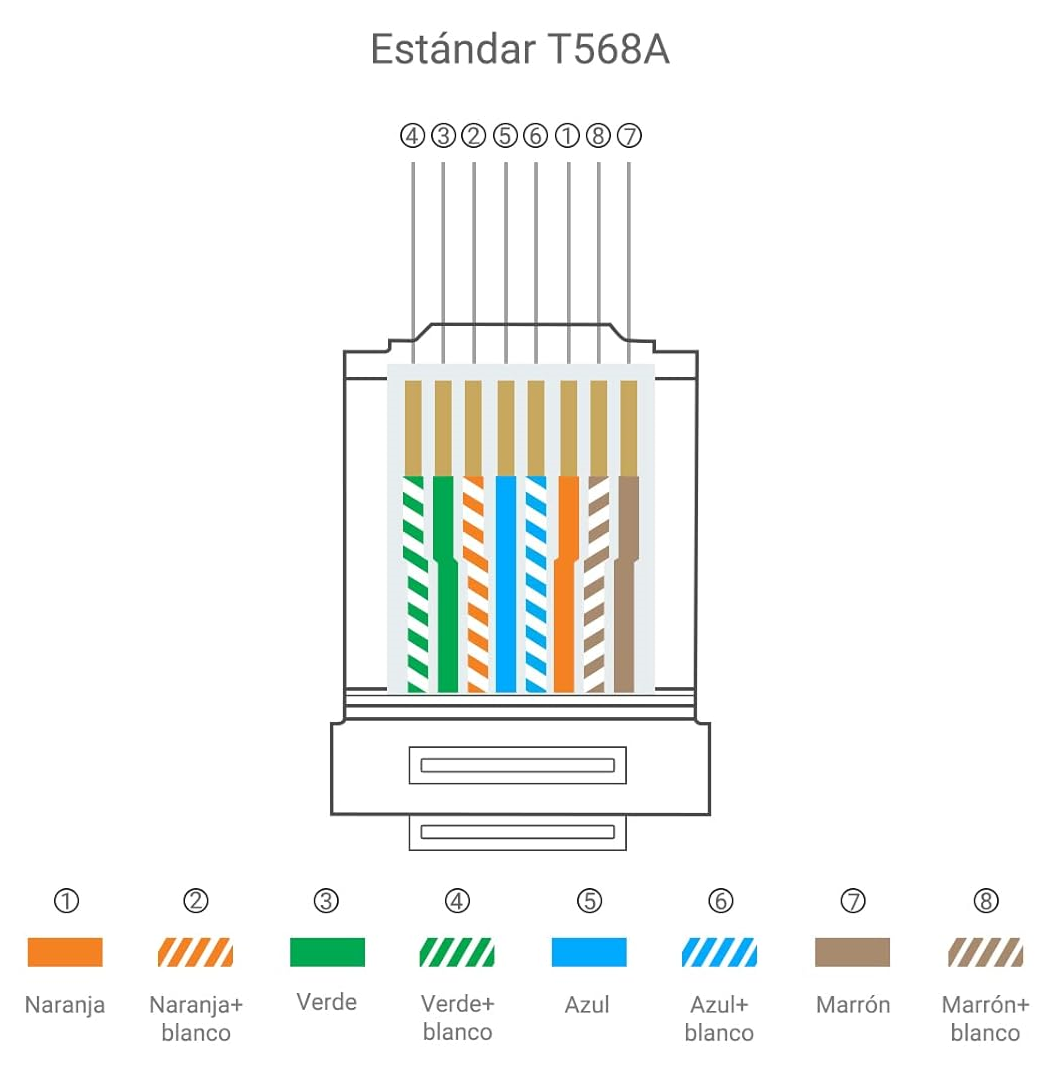
\includegraphics[width=\linewidth]{img/T568A.png}
            \caption{Estándar T568A.}
            \label{fig:estandar_t568a}
        \end{minipage}
        \begin{minipage}[b]{0.45\linewidth}
            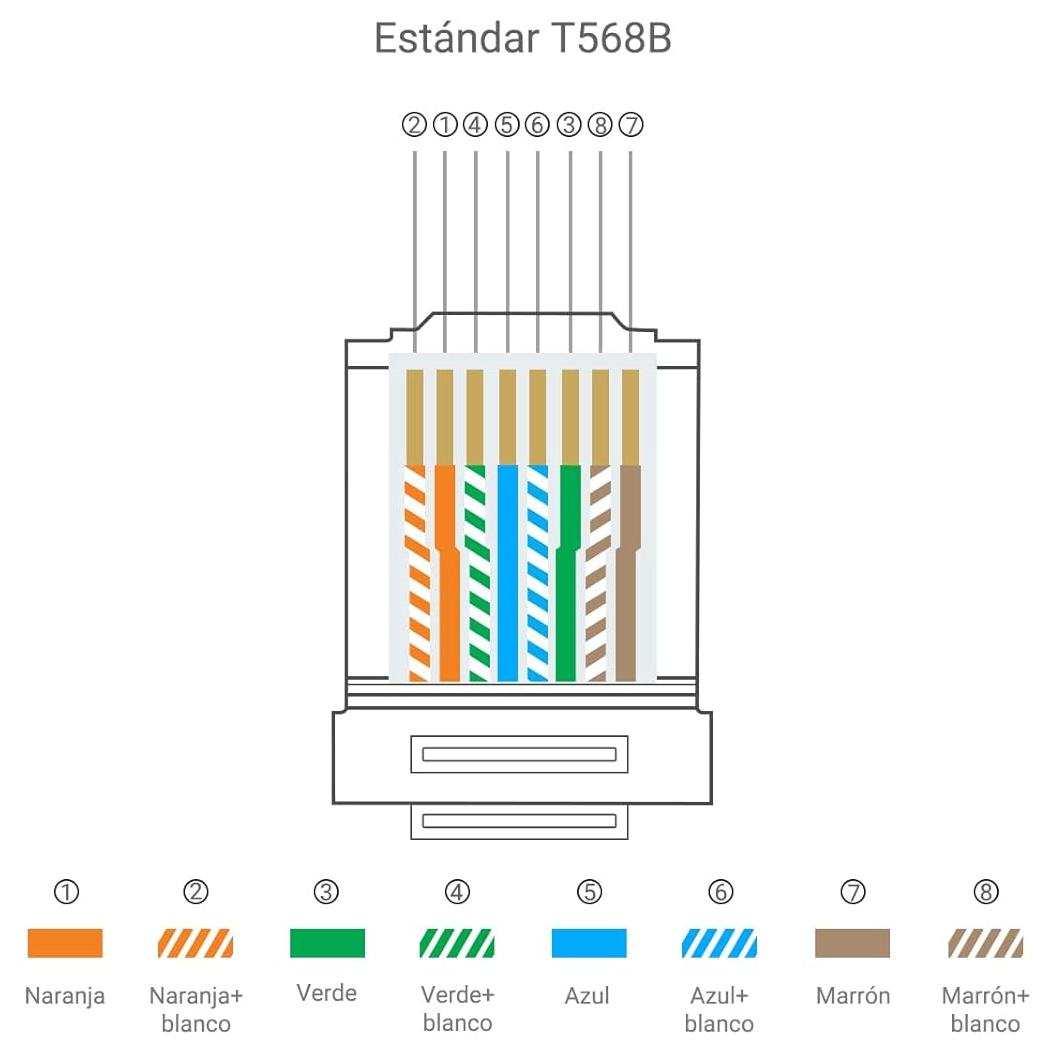
\includegraphics[width=\linewidth]{img/T568B.png}
            \caption{Estándar T568B.}
            \label{fig:estandar_t568b}
        \end{minipage}
    \end{figure}

    \newpage
\section{Desarrollo del trabajo}
    \subsection{Tarea 1: Espacio Físico}
        \subsubsection*{Paso 1}
        \textbf{Por equipo de trabajo, elabore una tabla y registre en ella los siguientes datos: Alumno, Número
        de PC, número de Rack y número de Patch Panel.}

        \begin{table}[H]
            \begin{center}
                \begin{tabular}{ l | c | c | c }
                    \textbf{Nombre} & \textbf{Número de PC} & \textbf{N. de Rack} & \textbf{N. de Patch Panel}\\ \hline
                    Luis Ángel Cruz Díaz & 14 & 29 & L302B1D14\\
                    Diego Alexis Moreno Valero & 13 & 29 & L302B1D13
                \end{tabular}
                \caption{Datos de los integrantes del equipo.}
                \label{tab:Datos_Equipo}
                \end{center}
        \end{table}

        \subsubsection*{Paso 2}
        \textbf{Haga un mapa del sitio e indique la trayectoria del cableado: desde la PC de cada integrante de su equipo, hasta el patch panel correspondiente; muestre en tal mapa los puntos de conexión y las longitudes. Para ello auxíliese de elementos gráficos.}

        La PC1 está ubicada en el Rack 29, en el Patch Panel L302B1D14. La PC2 está ubicada en el Rack 29, en el Patch Panel L302B1D13. En la figura \ref{fig:mapa_sitio} se muestra el mapa del sitio.

        \begin{figure}[H]
            \centering
            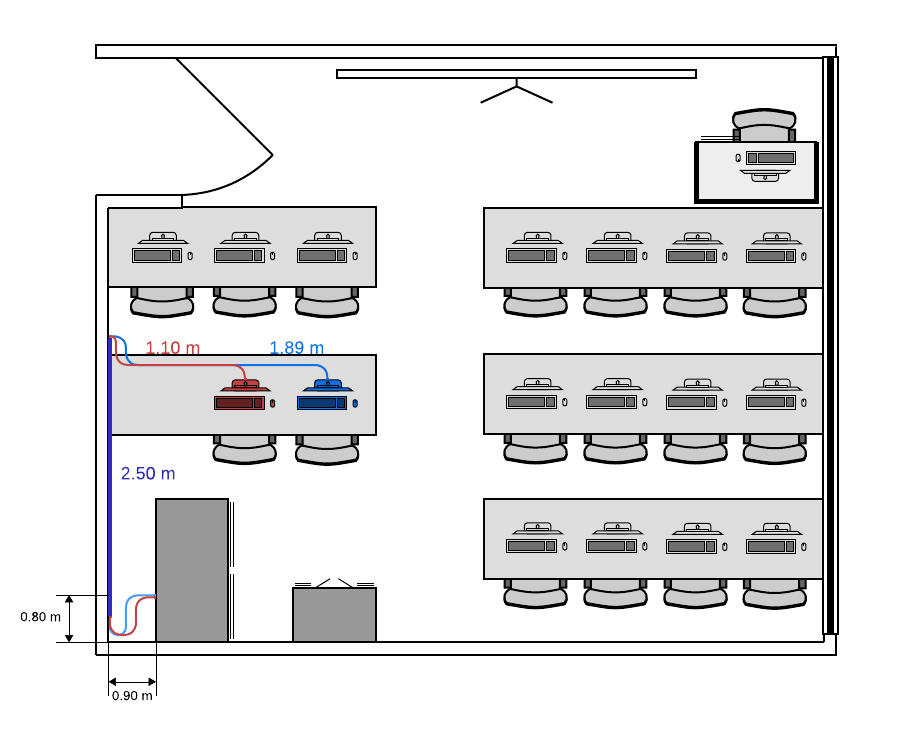
\includegraphics[width=0.8\textwidth]{img/planos.png}
            \caption{Mapa del sitio.}
            \label{fig:mapa_sitio}
        \end{figure}

    \subsection{Tarea 2: Construcción de Cables de Red}
        \subsubsection*{Paso 1}
        \textbf{Por equipo, de acuerdo a lo visto en clase, construya un cable recto y un cable cruzado.}
        \begin{enumerate}
            \item \textbf{¿Qué estándar(es) empleó para cada tipo de cable?}
            Se empleó los estándares T568A y T568B.
            \item \textbf{¿Qué categoría de cable utilizó?}
            Se utilizó cable de categoría 5e.
            \item \textbf{¿Qué tipo de conectores empleó?}
            Se emplearon conectores RJ45.
            \item \textbf{Explique por qué el cable UTP puede evitar el crosstalk.}
            El cable UTP evita el crosstalk (diafonía) gracias a la torsión de sus pares de hilos. Estos giros reducen las interferencias electromagnéticas entre los hilos dentro del mismo cable y con cables cercanos, minimizando la posibilidad de que las señales de un par interfieran con las de otro.
            \item \textbf{Explique qué problema podría suscitarse si no se emplea:}
            \begin{enumerate}
                \item \textbf{El estándar adecuado para cable recto y cruzado.}
                Es importante utilizar el estandar adecuado cuando se está utilizando equipos antiguos, ya que no soportan tecnologías como Auto-MDIX, que permite la conexión de dispositivos de red sin importar si el cable es recto o cruzado.
                \item \textbf{La categoría adecuada según el ancho de banda requerido.}
                El problema que podría suscitarse es que la velocidad de transmisión de datos no sea la adecuada para la aplicación que se requiere.
                \item \textbf{El tipo de conector de acuerdo a la categoría del cable.}
                El problema que podría suscitarse es que los cables del conector no se ajusten correctamente a los pines del conector RJ45, lo que podría ocasionar que la conexión no sea estable ya que los pines no estarían en contacto.
            \end{enumerate}
        \end{enumerate}

        \subsubsection*{Paso 2}
        \textbf{Desconecte, cada integrante, el cable de red de su PC y enciéndalas: una bajo Windows (PC1) y otra bajo Linux (PC2). Posteriormente:}

        \begin{enumerate}
            \item \textbf{Conecten un extremo del cable recto a la PC1. ¿Enciende algún LED de la tarjeta de red?}
            No, no enciende ningún LED de la tarjeta de red.
            \item \textbf{¿Qué muestra el ícono ``conexión de área loca'' en la PC1 (tache, símbolo de admiración, nada, otro)?}
            En la figura \ref{fig:cable_conectado} se observa que no muestra nada, no hay diferencia si el cable está conectado o no. Únicamente muestra el mensaje ``No conectado''.
            \begin{figure}[H]
                \centering
                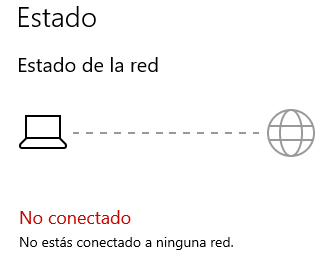
\includegraphics[width=0.5\textwidth]{img/cable_conectado.png}
                \caption{Cable conectado unicamente a la PC1.}
                \label{fig:cable_conectado}
            \end{figure}

            En el caso de Linux (PC2), no deja activar la conexión de red, ya que no detecta que haya un cable conectado a la tarjeta de red. En la figura \ref{fig:conexion_no_activa} se muestra que no se puede activar la conexión de red.

            \begin{figure}[H]
                \centering
                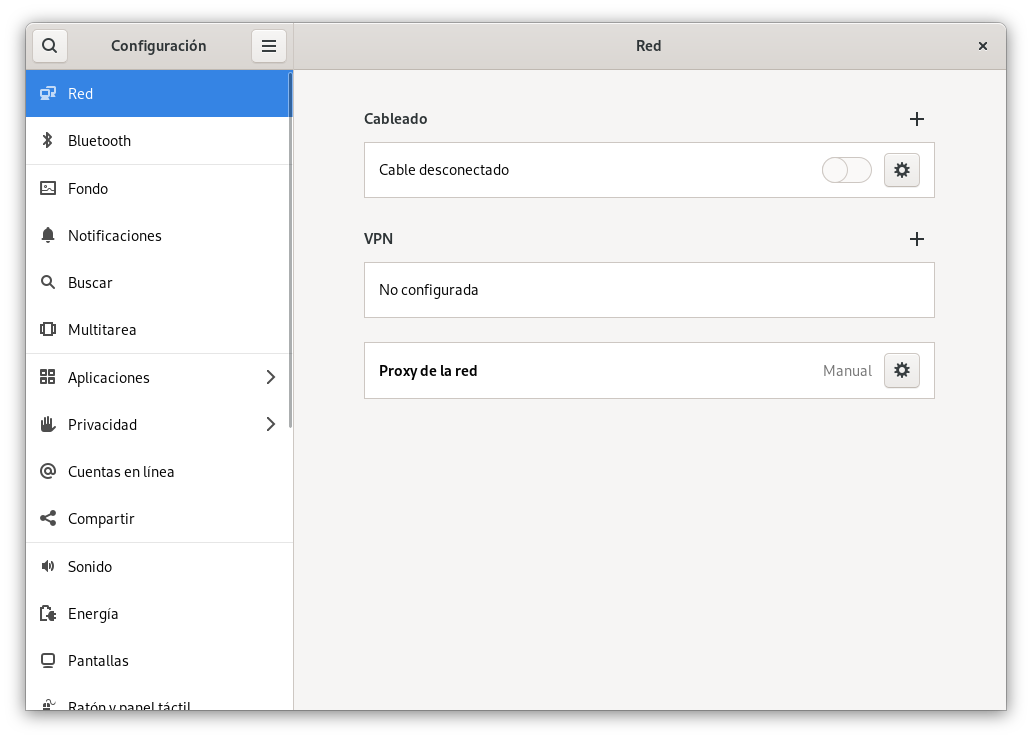
\includegraphics[width=0.5\textwidth]{img/Cable_desconectado_linux.png}
                \caption{Conexión de red no activa en Linux.}
                \label{fig:conexion_no_activa}
            \end{figure}

            \item \textbf{Ahora conecten el otro extremo a la PC2. ¿Encienden los LEDs de ambas tarjetas de red?}
            Si, encienden los LEDs de ambas tarjetas de red.
            \item \textbf{¿Qué muestra el ícono ``conexión de área local'' en la PC1 (tache, símbolo de admiración, nada, otro)?}
            En la figura \ref{fig:cable_conectado_ambas} aparece un conector RJ45, indicando que hay un cable conectado. El mensaje cambia a ``No hay acceso a Internet''.
            \begin{figure}[H]
                \centering
                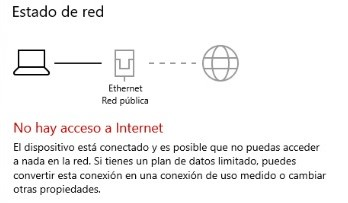
\includegraphics[width=0.5\textwidth]{img/cable_conectado_ambas.jpg}
                \caption{Cable conectado a ambas PCs.}
                \label{fig:cable_conectado_ambas}
            \end{figure}

            En el caso de Linux (PC2), se habilita la conexión de red, ya que detecta que hay un cable conectado a la tarjeta de red. En la figura \ref{fig:conexion_activa} se muestra que ahora se encuentra activa la conexión de red.

            \begin{figure}[H]
                \centering
                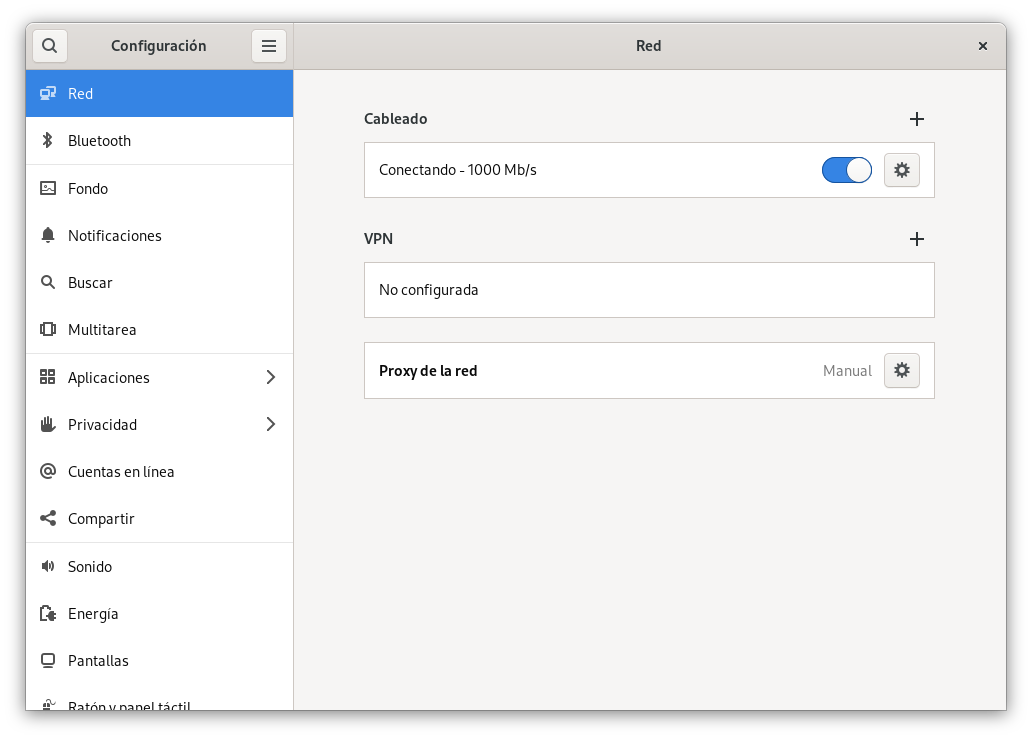
\includegraphics[width=0.5\textwidth]{img/cable_conectado_linux.png}
                \caption{Conexión de red activa en Linux.}
                \label{fig:conexion_activa}
            \end{figure}

            \item \textbf{Expliquen por qué ocurre tal situación en los puntos a y c}
            La luz indica que existe conexión física entre las tarjetas de red, al conectar el cable por un único extremo, no se establece la conexión física entre las tarjetas de red, por lo que no se encienden los LEDs. Al conectar ambos extremos, se establece la conexión física y se encienden los LEDs como indicador de que hay conexión.
            \item \textbf{Expliquen lo que nos dice el ícono que aparece en el punto b y en el punto d}
            En la figura \ref{fig:cable_conectado}, el ícono indica que no hay conexión física entre tarjetas de red, debido a que únicamente se conectó un extremo del cable. En la figura \ref{fig:cable_conectado_ambas}, el ícono indica que hay conexión física entre las tarjetas de red, ya que se conectaron ambos extremos del cable.
        \end{enumerate}

    \subsection{Tarea 3: Configuración de red bajo Windows y Linux}
    \textbf{Dejen conectado el cable cruzado entre las PCs y, a continuación, realicen y describan, textual y gráficamente, los pasos llevados a cabo para cumplir con el siguiente paso 1.}
        \subsubsection*{Paso 1}

        \textbf{Para cambiar la dirección IP, la máscara de subred y la puerta de enlace en la PC1, bajo Windows, se siguen los siguientes pasos:}

        \begin{enumerate} 
            \item Abre el \texttt{Panel de control}. 
            \item Selecciona \texttt{Centro de redes y recursos compartidos}. 
            \item Haz clic en \texttt{Cambiar configuración del adaptador}. 
            \item Elige la conexión de red que deseas configurar. 
            \item Haz clic en \texttt{Propiedades}. 
            \item Selecciona \texttt{Protocolo de Internet versión 4 (TCP/IPv4)}. 
            \item Marca la opción \texttt{Usar la siguiente dirección IP}. 
            \item Introduce la dirección IP, la máscara de subred y la puerta de enlace en los campos correspondientes. 
        \end{enumerate}

        En este caso se tomó \texttt{192.168.0.14} como dirección IP, \texttt{255.255.255.0} como mascara de subred y \texttt{192.168.0.1} como puerta de enlace, estos cambios se muestra en la figura~\ref{fig:cambiar_configuracion_red_windows}.

        \begin{figure}[H]
            \centering
            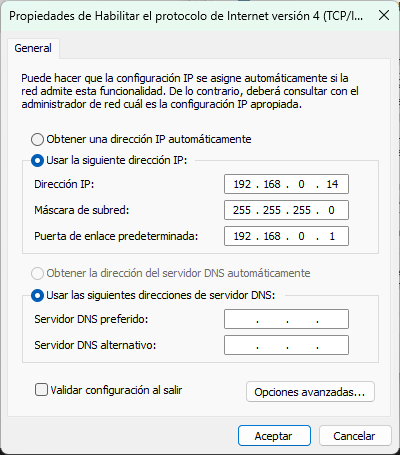
\includegraphics[width=0.4\textwidth]{img/cambiar_IP_Windows.png}
            \caption{Cambio de configuración de red en Windows.}
            \label{fig:cambiar_configuracion_red_windows}
        \end{figure}

        \textbf{Para cambiar la dirección IP, la máscara de subred y la puerta de enlace en la PC2, bajo Linux, se siguen los siguientes pasos:}

        \begin{enumerate}
            \item Abrir configuración de red.
            \item Seleccionar la conexión de red.
            \item Seleccionar la opción de configuración manual.
            \item Introducir la dirección IP, la máscara de subred y la puerta de enlace en los campos correspondientes.
        \end{enumerate}

        En este caso se tomó \texttt{192.168.0.13} como dirección IP, \texttt{255.255.255.0} como mascara de subred y \texttt{192.168.0.1} como puerta de enlace, estos cambios se muestra en la figura~\ref{fig:cambiar_configuracion_red_linux}.

        \begin{figure}[H]
            \centering
            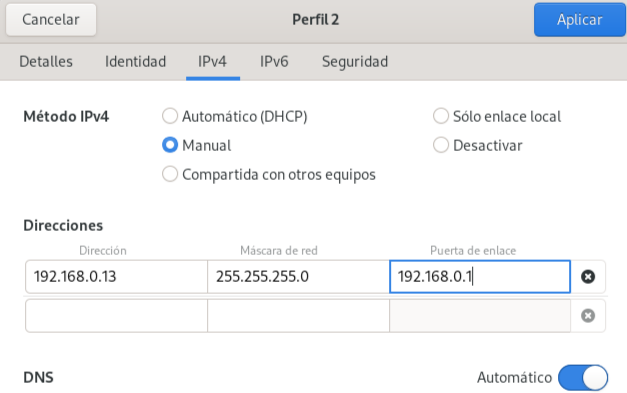
\includegraphics[width=0.6\textwidth]{img/cambiar_IP_Linux.png}
            \caption{Cambio en la configuración de red en Linux.}
            \label{fig:cambiar_configuracion_red_linux}
        \end{figure}

    \subsection{Tarea 4: Información de protocolos TCP/IP}
        \subsubsection*{Paso 1}

        Con los datos obtenidos, se llenó la tabla \ref{tab:informacion_tcpip} con la información de la PC1 y la PC2.

        \begin{table}[H]
            \begin{center}
                \begin{tabular}{ c | c | c}
                    \textbf{Datos} & \textbf{Computadora 1} & \textbf{Computadora 2} \\ \hline
                    \textbf{Dirección IP} & 192.168.0.14 & 192.168.0.13\\
                    \textbf{Máscara de subred} & 255.255.255.0 & 255.255.255.0\\
                    \textbf{Puerta de enlace} & 192.168.0.1 & 192.168.0.1\\
                \end{tabular}
                \caption{Dirección IP, Máscara de subred y Puerta de enlace de las computadoras.}
                \label{tab:informacion_tcpip}
                \end{center}
        \end{table}

        En la PC1, bajo Windows, ejecutó el comando \texttt{ipconfig} en la consola de comandos, en la figura \ref{fig:ipconfig_windows} se muestra la información de red.

        \begin{figure}[H]
            \centering
            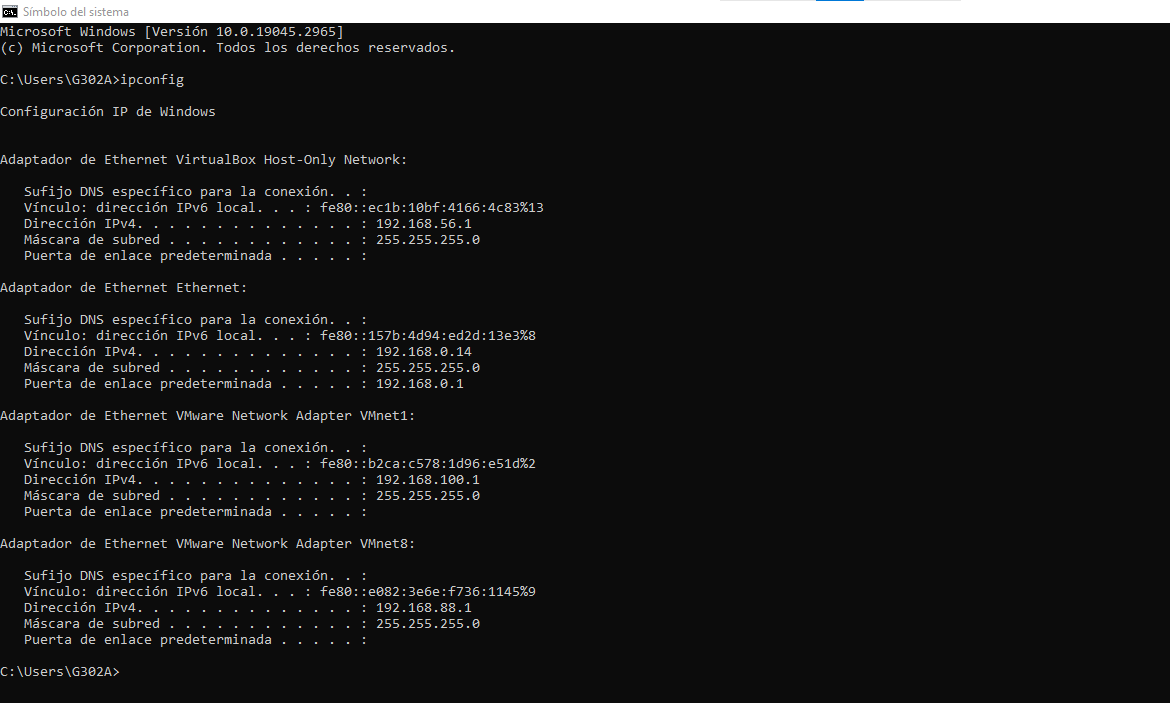
\includegraphics[width=0.6\textwidth]{img/ipconfig_windows.png}
            \caption{Información de red en Windows con el comando \texttt{ipconfig}.}
            \label{fig:ipconfig_windows}
        \end{figure}

    \subsection{Tarea 5: Conectividad}
        \subsubsection*{Paso 1}
        
        En windows, se ejecutó el comando \texttt{ping} hacia la PC2, en la figura \ref{fig:ping_windows} se muestra la respuesta que se obtuvo al ejecutar el comando.

        \begin{figure}[H]
            \centering
            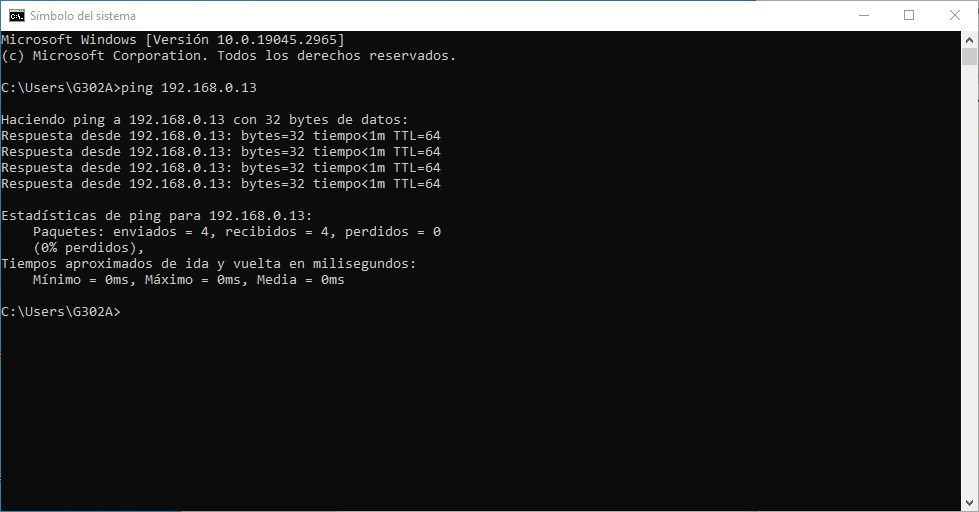
\includegraphics[width=0.6\textwidth]{img/PC1_a_PC2.jpg}
            \caption{Ping de Windows a Linux.}
            \label{fig:ping_windows}
        \end{figure}

        \begin{enumerate}
            \item \textbf{¿Hay respuesta de la PC2 a la PC1?}
            Si, hay respuesta.
            \item \textbf{¿Qué mensaje envían?}
            Al ejecutar el comando \texttt{ping} desde la PC1 hacia la PC2, se envían paquetes de datos a la PC2 y se recibe una respuesta de la misma de que los paquetes fueron recibidos.
        \end{enumerate}

        \subsubsection*{Paso 2}
        
        En Linux, se ejecutó el comando \texttt{ping} hacia la PC1 utilizando la bandera \texttt{-c 4} para enviar únicamente 4 paquetes de datos.

        \begin{enumerate}
            \item \textbf{¿Hay respuesta de la PC1 a la PC2?}
            Si, hay respuesta.
            \item \textbf{¿Qué mensaje envían?}
            Al ejecutar el comando \texttt{ping} desde la PC2 hacia la PC1, se envían paquetes de datos a la PC1 y se recibe una respuesta de la misma de que los paquetes fueron recibidos.
        \end{enumerate}

        En caso de que no exista conectividad en alguno de los dos pasos anteriores, informe al profesor y repítalo. 

        \subsubsection*{Paso 3}
        Explique si hubo que modificar alguna configuración en las PCs para tener repuesta en el ping

        En Windows debe activarse la opción de ``Archivos e impresoras compartidos (petición eco: ICMPv4)'' en el Firewall de Windows. En la figura \ref{fig:activar_ping} se muestra cómo se tiene habilidado esta opción.

        \begin{figure}[H]
            \centering
            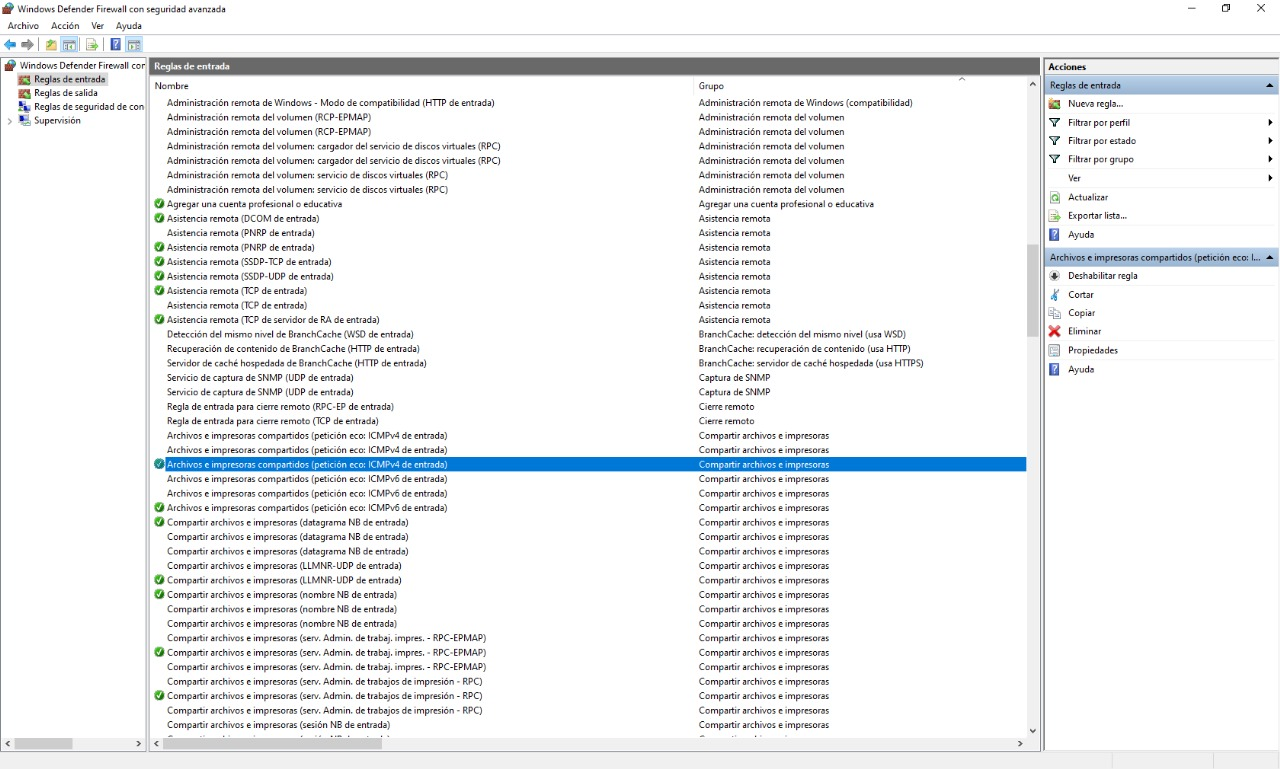
\includegraphics[width=0.6\textwidth]{img/firewall.jpg}
            \caption{Activar petición eco en Windows.}
            \label{fig:activar_ping}
        \end{figure}

\section{Observaciones}

    En algunas PC's con Windows, es necesario habilitar la opción de ``Archivos e impresoras compartidos (petición eco: ICMPv4)'' en el Firewall de Windows para poder realizar el ping entre las computadoras, ya que por defecto esta opción se encuentra deshabilitada. Si no se habilita esta opción, no se podrá realizar la conexión entre las computadoras, mandando que los paquetes enviados con el comando \texttt{ping} se pierdan.

\section{Conclusiones}

    \begin{itemize}
    \item Luis Ángel Cruz Díaz - 2183038433\\
        En esta práctica aprendimos a hacer cables de red rectos y cruzados siguiendo los estándares T568A y T568B. También configuramos las direcciones IP y las máscaras de red en dos computadoras, una con Windows y otra con Linux. Después, verificamos que las computadoras pudieran comunicarse directamente usando un cable. Descubrimos que era necesario activar la opción de ``Archivos e impresoras compartidos (petición eco: ICMPv4)'' en el Firewall de Windows para poder hacer ping entre ellas.
    \item Diego Alexis Moreno Valero - 2243900185\\
    \end{itemize}

% --- Para agregar un apéndice
%\newpage
%\appendix
%\appendixpage
%\addappheadtotoc
%\section{Nombre del apéndice}